\documentclass[12pt]{article}
\usepackage{fullpage}

\usepackage[T1]{fontenc}
\usepackage[utf8]{inputenc}
\usepackage{lmodern}
\usepackage{microtype}
\usepackage[full]{textcomp}
\usepackage[osf]{newtxtext}
\usepackage{graphicx}

%% ---- Base math packages (always available) -------------------------------
\usepackage{amsmath, amssymb, amsthm, mathtools}
\usepackage{hyperref}

%% ---- Submission preamble (imported so the inlined solution compiles) ----
\usepackage{amsmath,amssymb,amsthm,mathtools}

\newtheorem{theorem}{Theorem}[section]
\newtheorem{proposition}[theorem]{Proposition}
\newtheorem{lemma}[theorem]{Lemma}
\theoremstyle{definition}
\newtheorem{definition}[theorem]{Definition}
\theoremstyle{remark}
\newtheorem{remark}[theorem]{Remark}

\newcommand{\Aut}{\operatorname{Aut}}
\newcommand{\rng}{\operatorname{rng}}
\newcommand{\dom}{\operatorname{dom}}

%% ---- Theorem environments not supplied by the submission ------------------
\makeatletter
\@ifundefined{theorem}{\newtheorem{theorem}{Theorem}}{}
\@ifundefined{lemma}{\newtheorem{lemma}{Lemma}}{}
\@ifundefined{proposition}{\newtheorem{proposition}{Proposition}}{}
\@ifundefined{corollary}{\newtheorem{corollary}{Corollary}}{}
\@ifundefined{definition}{\theoremstyle{definition}\newtheorem{definition}{Definition}}{}
\@ifundefined{remark}{\theoremstyle{remark}\newtheorem{remark}{Remark}}{}
\makeatother

%% ---- First Proof theme + in-text comment box -----------------------------
%% Palette from the FINAL DELIVERABLES brand assets:
%%   slate     #171313  (ink)
%%   warm-gray #69626D  (secondary)
%%   sand      #F2ECE9  (light background)
\usepackage{xcolor}
\usepackage[most]{tcolorbox}

\definecolor{FPslate}{HTML}{171313}
\definecolor{FPwarmgray}{HTML}{69626D}
\definecolor{FPsand}{HTML}{F2ECE9}

% Reviewer number for this document (set per file). Used by the comment box tag.
\newcommand{\reviewernum}{1}

% \review{...} : a First-Proof-themed reviewer comment, set inline in the text
%            as a sand box with a warm-gray rule and a "Reviewer N" tag.
\newtcolorbox{reviewbox}{
  breakable, enhanced, sharp corners,
  colback=FPsand, colframe=FPwarmgray,
  coltext=FPslate, boxrule=0pt, leftrule=2.5pt,
  left=8pt, right=8pt, top=14pt, bottom=5pt,
  before skip=6pt, after skip=6pt,
  fontupper=\small,
  overlay unbroken and first={
    \node[anchor=north east, font=\bfseries\footnotesize\sffamily,
          text=FPwarmgray, inner sep=0pt]
      at ([xshift=-8pt,yshift=-4pt]frame.north east) {Reviewer~\reviewernum};}
}
\newcommand{\review}[1]{\begin{reviewbox}#1\end{reviewbox}}

\title{Review of Submission 1B}
\author{First Proof Second Batch \\ Reviewer \reviewernum}
\date{June 4--8, 2026}

\makeatletter
\renewcommand{\maketitle}{%
  \noindent
  \begin{minipage}[t]{0.68\textwidth}
    \vspace{20pt}
    \raggedright
    {\LARGE\bfseries \@title\par}
    \vspace{0.35em}
    {\large \@author\par}
    \vspace{0.35em}
    {\normalsize \@date\par}
  \end{minipage}%
  \hfill
  \begin{minipage}[t]{0.25\textwidth}
    \vspace{0pt}
    \raggedleft
    \raisebox{\dimexpr-\height+\ht\strutbox+0.225in\relax}{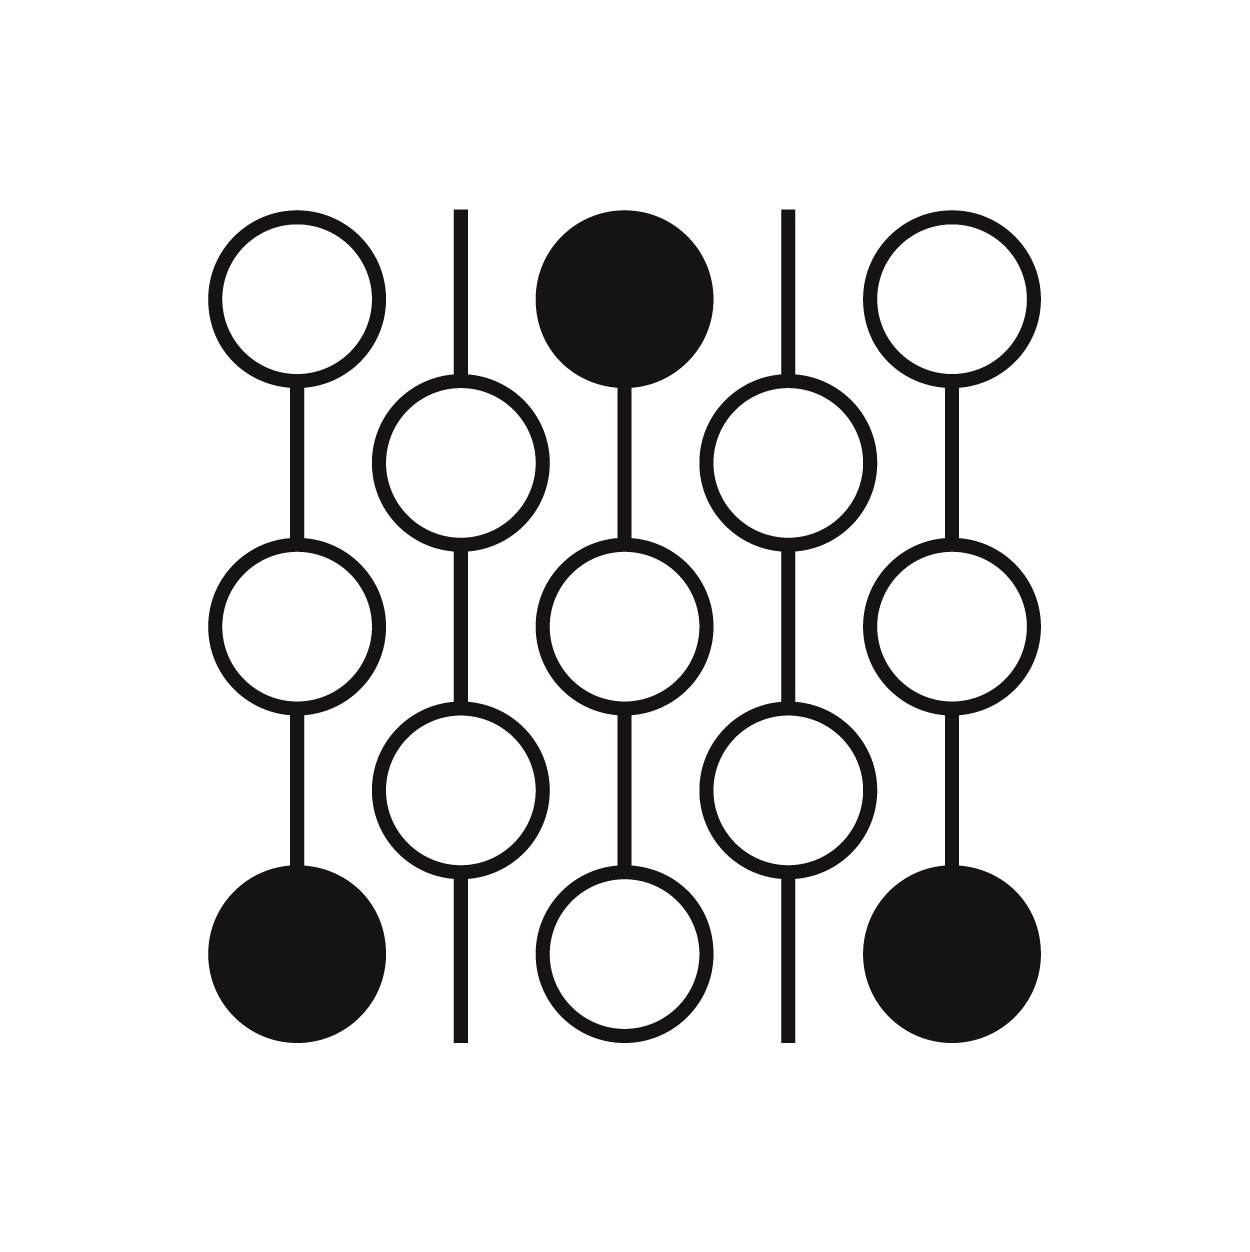
\includegraphics[height=1.35in]{Logo-slate.png}}
  \end{minipage}
  \par\vspace{2em}
}
\makeatother

\begin{document}
\maketitle
\section{Review}
%

\paragraph{Correctness.}
As far as I can tell, this solution is completely correct.

\paragraph{Novelty.}

This solution is very similar to one of the other AI solutions (with some essentially cosmetic differences), so I will reproduce here some of the comments I made in my review of that solution, which mostly apply equally well to both.
\begin{quote}
    This solution is highly reminiscent of a construction introduced by Dan Turetsky in the paper ``Coding in the automorphism group of a countable structure'' and subsequently used in at least two other papers. It is most similar to a version of Turetsky's technique used in the proof of Theorem 4.6 of the paper ``Scott complexity of countable structures'' by Rachel Alvir, Noam Greenberg, Matthew Harrison-Trainor and Dan Turetsky. In particular, the structure $\mathcal{A}$ constructed in the solution below is very similar to the structure constructed by Alvir, Greenberg, Harrison-Trainor and Turetsky, although the purpose it is being used for and the verification that it has the desired properties are somewhat different. I would like to note that this similarity was pointed out to me by another referee, after which I independently verified that the two constructions are indeed highly similar.

    It would be interesting to know to what extent the AI system that composed this solution was aware of these papers and, furthermore, to what extent they directly inspired its solution. One piece of evidence which is suggestive, but not definitive, is that some of the notation in the solution below is fairly similar to that used by Turetsky and by Alvir, Greenberg, Harrison-Trainor and Turetsky. For example, in all three, an arbitrary countable infinite dimensional $\mathbb{F}_2$ vector space is needed and the particular one chosen is $([\omega]^{<\omega}, \Delta)$ (i.e.\ the set of finite sets of natural numbers with the operation of symmetric difference playing the role of vector space addition). This choice is slightly unusual, though perhaps somewhat less so in computability theory than in some other fields. Furthermore, in both Turetsky's paper and the solution below, an infinite number of auxiliary sets are needed and in both cases they are referred to as $\{V_n\}_n$. These similarities constitute moderate evidence that the AI system may have been aware of one or both of these papers when devising its solution but fall far short of definitive evidence for this possibility.

    If I encountered the solution below as part of a paper I was referring for a journal, I would insist that the authors cite the work of Turetsky and point out the similarity in the constructions, but I would also consider the solution below to be a minor, but novel and interesting variation on Turetsky's technique.
\end{quote}
I should point out that one of the points above is not quite accurate for this solution. In particular, while this solution does have an auxiliary set which is denoted $V$, it does not have an infinite sequence of auxiliary sets (or, more precisely, it does, but they are no longer explicitly demarcated). However, there are certain other ways in which this solution is more similar to Turetsky's construction than the solution discussed in the quote above. Overall, my judgment is similar: there is suggestive, but not definitive, evidence that the AI system was inspired by Turetsky's work.

\paragraph{Exposition.}
The style in which this solution is written is rather strange. 

First, it is extremely pedantic and insists on spelling out details that are usually left implicit. For example, it explicitly describes how to represent finite sets of natural numbers by individual natural numbers and then proves various facts about this representation which should be self-evident to any professional mathematician. This tendency increases the amount of notation required throughout the solution, which sometimes makes the solution more difficult to read (since one has to keep track of more variable names and more notation). It also sometimes leads to one or more paragraphs in a row spent proving things that are very obvious and extremely tangential to the main ideas of the solution.

Another odd feature of the exposition is a tendency to use terms in somewhat non-standard ways. For example, the solution repeatedly refers to pairs of chains as ``gadgets'' (a term which is sometimes used in mathematics and theoretical computer science but is usually used for more combinatorially complicated objects) and talks about formulas being ``preserved and reflected'' by embeddings (rather than just preserved).

Finally, the solution begins with a section called ``Overview/Strategy'' which contains a technically accurate but extremely opaque high-level description of the solution. My experience was that before reading the rest of the solution, I had little idea what this section was trying to say, but after reading the entire solution (at which point an ``overview'' section is no longer especially helpful) I understood what each sentence was intended to communicate.

In spite of these odd features, however, the solution is not especially hard to read and is reasonably well-organized.

% strange overview section
% referring to things as "gadgets", "preserved and reflected"

\section{Recommendation}
Essentially flawless, but with one major caveat. As I wrote in my review of another, similar, AI solution:
\begin{quote}
If the AI system was aware of---and especially if it was directly inspired by---Turetsky's work as discussed above, then its failure to cite or even mention Turetsky (or any of the papers which use his technique) is a serious and very concerning oversight. It seems reasonable likely that this occurred, but not certain.
\end{quote}


  \section{Submission with inline comments}

%% ======================================================================
%% Inlined verbatim from the anonymised submission prob_001-B.
%% ======================================================================
%
\date{}


\subsection*{Overview / Strategy}

We build a computable structure in a finite relational language with three sorts.  The first sort is a rigid successor ray of labels.  The second sort codes finite subsets of the label set, with a relation \(Q\) that toggles one label at a time.  The third sort places, above each label, two directed successor rays.  The finite subset coded on the second sort determines which pairs of rays are swapped.  Sections~\ref{sec:construction} and~\ref{sec:automorphisms} give the construction and prove that the automorphisms are exactly the finite toggles.

The copy-computability argument is nonuniform in the automorphism, as required by Turing reducibility: for a given copy and a given automorphism, the finite support and finitely many roots can be hardwired into an oracle program using the atomic diagram of the copy.  This is proved in Section~\ref{sec:copies}.  Finally, Section~\ref{sec:nondef} proves nondefinability.  Given any finite parameter tuple, we choose a fresh two-ray gadget.  The automorphism swaps the two rays of that gadget, while an injective shift of one ray preserves and reflects all atomic facts and fixes the parameters.  Existential formulas true of the genuine graph pair therefore remain true of a false pair, ruling out any \(\Sigma^{\mathrm{in}}_1\)-definition of that automorphism from the allowed parameters.

\subsection{Definitions and the headline theorem}

Throughout, \(\omega=\mathbb N\).  A copy of a countable structure means a structure with domain \(\omega\).  If \(\mathcal B\) is a structure in a finite relational language, \(D(\mathcal B)\) denotes its complete atomic diagram; equivalently, up to Turing equivalence, it is the finite join of the characteristic functions of the basic relations of \(\mathcal B\).

\begin{definition}
Let \(\mathcal M\) be a countable structure with domain \(\omega\).
\begin{enumerate}
\item \(\mathcal M\) is \emph{computably \(\operatorname{AUT}\)-countable} if every \(\rho\in\Aut(\mathcal M)\) satisfies \(\rho\leq_T D(\mathcal M)\).
\item \(\mathcal M\) is \emph{computably \(\operatorname{AUT}\)-countable on a cone} if there is \(C\subseteq\omega\) such that for every copy \(\mathcal B\cong\mathcal M\) with domain \(\omega\), every \(\rho\in\Aut(\mathcal B)\) satisfies \(\rho\leq_T D(\mathcal B)\oplus C\), where \(\oplus\) is Turing join.
\end{enumerate}
\end{definition}

\begin{definition}
An existential formula is a formula of the form
\[
\exists z_0\cdots \exists z_{n-1}\,\theta,
\]
where \(n<\omega\) and \(\theta\) is quantifier-free.  In the final nondefinability argument we prove the stronger statement allowing \(\theta\) to be a quantifier-free \(L_{\omega_1\omega}\)-formula built from atomic formulas by negation and countable conjunctions and disjunctions.

Let \(P\subseteq M\) be finite.  A function \(f:M\to M\) is \emph{\(\Sigma^{\mathrm{in}}_1\)-definable in \(\mathcal M\) over parameters from \(P\)} if there is a countable family \((\varphi_i(x,y))_{i\in\omega}\) of existential formulas, each using only parameters from \(P\), such that for all \(x,y\in M\),
\[
f(x)=y
\quad\Longleftrightarrow\quad
\mathcal M\models \varphi_i(x,y)\text{ for some }i\in\omega.
\]
\end{definition}

\begin{theorem}[Headline theorem: positive answer to the original problem]\label{thm:main}
There is a computable structure \(\mathcal A\) with domain \(\omega\), in a finite relational language, such that:
\begin{enumerate}
\item For every copy \(\mathcal B\cong\mathcal A\) with domain \(\omega\), every automorphism of \(\mathcal B\) is computable relative to \(D(\mathcal B)\).  Thus \(\mathcal A\) is computably \(\operatorname{AUT}\)-countable on a cone with cone base \(\emptyset\).
\item For every finite tuple \(\bar a\) from \(\mathcal A\), there is an automorphism \(\pi\in\Aut(\mathcal A)\) such that \(\pi\) is not \(\Sigma^{\mathrm{in}}_1\)-definable in \(\mathcal A\) over parameters from
\[
\rng(\bar a)\cup \pi[\rng(\bar a)].
\]
\end{enumerate}
\end{theorem}

\begin{proof}
The structure is constructed and proved computable in Proposition~\ref{prop:construction}.  Proposition~\ref{prop:copies} proves clause~(1).  Proposition~\ref{prop:nondef} proves clause~(2), indeed with quantifier-free infinitary matrices allowed in the existential formulas.  These propositions concern the same structure \(\mathcal A\), so together they prove the theorem.
\end{proof}

\subsection{Construction of the computable structure}\label{sec:construction}

Fix a computable pairing bijection \(\langle\cdot,\cdot\rangle:\omega^2\to\omega\) with computable projections.  For \(e\in\omega\), let
\[
F_e=\{i\in\omega:\text{the \(i\)-th binary digit of \(e\) is \(1\)}\}.
\]
Thus \(F_e\) is finite, and every finite \(F\subseteq\omega\) has the unique code
\[
c(F)=\sum_{i\in F}2^i
\]
with \(F_{c(F)}=F\).

For \(l,e,k\in\omega\) and \(b\in\{0,1\}\), put
\[
\lambda_l=3l,\qquad u_e=3e+1,\qquad v_{l,b,k}=3\langle l,2k+b\rangle+2.
\]
The language is the finite relational language
\[
\tau=\{L,U,V,N,I,Q,S,T\},
\]
where \(L,U,V\) are unary, \(N,I\) are binary, and \(Q,S,T\) are ternary.

Define a \(\tau\)-structure \(\mathcal A\) with domain \(\omega\) as follows.  The sort predicates are
\[
L^{\mathcal A}=\{\lambda_l:l\in\omega\},\quad
U^{\mathcal A}=\{u_e:e\in\omega\},\quad
V^{\mathcal A}=\{v_{l,b,k}:l,k\in\omega,\ b\in\{0,1\}\}.
\]
The remaining relations hold exactly in the following displayed cases:
\[
N(\lambda_l,\lambda_m)\Longleftrightarrow m=l+1,
\]
\[
I(\lambda_l,v_{m,b,k})\Longleftrightarrow l=m,
\]
\[
Q(\lambda_l,u_e,u_{e'})\Longleftrightarrow F_{e'}=F_e\triangle\{l\},
\]
\[
S(\lambda_l,v_{l,b,k},v_{l,b,k+1})
\quad\text{for all }l,b,k,
\]
and
\[
T(\lambda_l,u_e,v_{m,b,k})
\Longleftrightarrow
m=l\text{ and }b=\chi_{F_e}(l),
\]
where \(\triangle\) is symmetric difference and \(\chi_F\) is the characteristic function of \(F\).  For later use, write
\[
R_{l,b}=\{v_{l,b,k}:k\in\omega\},
\qquad
P_l=R_{l,0}\cup R_{l,1}.
\]

\begin{proposition}\label{prop:construction}
The structure \(\mathcal A\) is a computable structure with domain \(\omega\) in the finite relational language \(\tau\).  Moreover, \(L^{\mathcal A}\), \(U^{\mathcal A}\), and \(V^{\mathcal A}\) partition \(\omega\).
\end{proposition}

\begin{proof}
The three displayed sets lie in the three different congruence classes modulo \(3\), so they are pairwise disjoint.  If \(n\equiv 0\pmod 3\), then \(n=\lambda_{n/3}\).  If \(n\equiv 1\pmod 3\), then \(n=u_{(n-1)/3}\).  If \(n\equiv 2\pmod 3\), let \(q=(n-2)/3\).  The computable projections of the pairing function give unique \(l,t\) with \(q=\langle l,t\rangle\), and \(t\) has a unique form \(2k+b\) with \(b\in\{0,1\}\); hence \(n=v_{l,b,k}\).  Thus the three sorts partition \(\omega\), and membership in each sort is computable.

The relations are decidable from the displayed coordinates.  For \(N\), one checks that both arguments are labels and then compares their indices.  For \(I\), one checks that the first argument is a label and the second is a \(V\)-element and compares the label coordinates.  For \(Q\), one checks that the arguments have forms \(\lambda_l,u_e,u_{e'}\) and then decides whether the binary digits of \(e'\) are obtained from those of \(e\) by flipping exactly the \(l\)-th bit.  For \(S\), one checks that the arguments have the form \(\lambda_l,v_{l,b,k},v_{l,b,j}\) and then tests \(j=k+1\).  For \(T\), one checks that the arguments have the form \(\lambda_l,u_e,v_{m,b,k}\) and then tests \(m=l\) and whether the \(l\)-th binary digit of \(e\) is \(b\).  Hence every basic relation is computable, so \(\mathcal A\) is computable.
\end{proof}

\subsection{Classification of automorphisms}\label{sec:automorphisms}

For a finite \(F\subseteq\omega\), define \(\alpha_F:\omega\to\omega\) by
\[
\alpha_F(\lambda_l)=\lambda_l,\qquad
\alpha_F(u_e)=u_{c(F_e\triangle F)},\qquad
\alpha_F(v_{l,b,k})=v_{l,b\oplus\chi_F(l),k},
\]
where \(\oplus\) is addition modulo \(2\).

\begin{lemma}\label{lem:alpha-auto}
For every finite \(F\subseteq\omega\), \(\alpha_F\in\Aut(\mathcal A)\).
\end{lemma}

\begin{proof}
The map \(\alpha_F\) is an involution: toggling \(F\) twice restores each \(U\)-element, and adding \(\chi_F(l)\) modulo \(2\) twice restores each side of each \(V\)-gadget.  Hence it is bijective.  It preserves \(L,U,V\) setwise.  It fixes all labels, so it preserves \(N\).  It does not change the label coordinate of any \(V\)-element, so it preserves \(I\).

For \(S\), if \(S(\lambda_l,v_{l,b,k},v_{l,b,k+1})\) holds, then after applying \(\alpha_F\) we get
\[
S(\lambda_l,v_{l,b\oplus\chi_F(l),k},v_{l,b\oplus\chi_F(l),k+1}),
\]
which holds.  For \(Q\), if \(Q(\lambda_l,u_e,u_{e'})\) holds, then
\[
F_{e'}=F_e\triangle\{l\}.
\]
The two images in the \(U\)-sort code \(F_e\triangle F\) and \(F_{e'}\triangle F\), and
\[
F_{e'}\triangle F=(F_e\triangle\{l\})\triangle F=(F_e\triangle F)\triangle\{l\},
\]
so \(Q\) is preserved.  For \(T\), if \(T(\lambda_l,u_e,v_{m,b,k})\) holds, then \(m=l\) and \(b=\chi_{F_e}(l)\).  The image of \(u_e\) codes \(F_e\triangle F\), and the image side is
\[
b\oplus\chi_F(l)=\chi_{F_e}(l)\oplus\chi_F(l)=\chi_{F_e\triangle F}(l),
\]
so \(T\) is preserved.  Since \(\alpha_F\) is an involution, preservation of each relation implies reflection as well.  Thus \(\alpha_F\) is an automorphism.
\end{proof}

\begin{lemma}\label{lem:all-aut}
Every automorphism of \(\mathcal A\) is \(\alpha_F\) for a unique finite \(F\subseteq\omega\).
\end{lemma}

\begin{proof}
Let \(\beta\in\Aut(\mathcal A)\).  First, \(\beta\) fixes every label.  The element \(\lambda_0\) is the unique \(L\)-element with no \(N\)-predecessor, so \(\beta(\lambda_0)=\lambda_0\).  If \(\beta(\lambda_l)=\lambda_l\), then \(\lambda_{l+1}\) is the unique \(N\)-successor of \(\lambda_l\), so \(\beta(\lambda_{l+1})=\lambda_{l+1}\).  Induction gives \(\beta(\lambda_l)=\lambda_l\) for all \(l\).

For \(l\in\omega\), let \(\tau_l:U^{\mathcal A}\to U^{\mathcal A}\) be the toggle map
\[
\tau_l(u_e)=u_{c(F_e\triangle\{l\})}.
\]
For every \(u\in U^{\mathcal A}\), \(Q(\lambda_l,u,\tau_l(u))\) holds, and the third entry satisfying this formula is unique.  Since \(\beta\) fixes \(\lambda_l\) and preserves \(Q\),
\[
\beta(\tau_l(u))=\tau_l(\beta(u)).
\]
Let \(\beta(u_0)=u_d\) and put \(F=F_d\).  If \(F_e=\{l_0,\dots,l_{n-1}\}\), then
\[
u_e=\tau_{l_0}\cdots\tau_{l_{n-1}}(u_0).
\]
Using the commutation relation above,
\[
\beta(u_e)
=\tau_{l_0}\cdots\tau_{l_{n-1}}(u_d)
=u_{c(F_e\triangle F)}.
\]

It remains to analyze the \(V\)-sort.  Because \(\beta\) fixes each \(\lambda_l\) and preserves \(I\), it maps \(P_l\) onto itself.  On \(P_l\), the binary relation \(S(\lambda_l,\cdot,\cdot)\) is exactly the disjoint union of the two directed rays
\[
v_{l,b,0}\to v_{l,b,1}\to v_{l,b,2}\to\cdots
\qquad (b=0,1).
\]
The two roots \(v_{l,0,0}\) and \(v_{l,1,0}\) are exactly the elements of \(P_l\) with no \(S(\lambda_l,\cdot,\cdot)\)-predecessor.  Thus \(\beta\) either fixes the two roots or swaps them.  Since every element has a unique successor on its ray, the image of a root determines the image of the whole ray.  Hence for each \(l\) there is \(\epsilon_l\in\{0,1\}\) such that
\[
\beta(v_{l,b,k})=v_{l,b\oplus\epsilon_l,k}
\quad\text{for all }b,k.
\]
Now \(T(\lambda_l,u_0,v_{l,0,0})\) holds.  Applying \(\beta\) gives
\[
T(\lambda_l,u_d,v_{l,\epsilon_l,0}),
\]
so \(\epsilon_l=\chi_{F_d}(l)=\chi_F(l)\).  Therefore \(\beta\) agrees with \(\alpha_F\) on \(L\), \(U\), and \(V\).  Uniqueness follows because \(F\) is recovered from \(\beta(u_0)=u_{c(F)}\).
\end{proof}

Consequently,
\[
\Aut(\mathcal A)=\{\alpha_F:F\subseteq\omega\text{ finite}\}.
\]
In particular, the automorphism group is countable, and in the displayed computable copy each automorphism is computable, with its finite support hardwired.

\subsection{Automorphisms of arbitrary copies are computable from the copy}\label{sec:copies}

\begin{proposition}\label{prop:copies}
Let \(\mathcal B\cong\mathcal A\) be any copy with domain \(\omega\).  If \(\rho\in\Aut(\mathcal B)\), then \(\rho\leq_T D(\mathcal B)\).  Hence \(\mathcal A\) is computably \(\operatorname{AUT}\)-countable on a cone with cone base \(\emptyset\).
\end{proposition}

\begin{proof}
Choose an isomorphism \(h:\mathcal A\to\mathcal B\).  Then \(h^{-1}\rho h\in\Aut(\mathcal A)\), so by Lemma~\ref{lem:all-aut} there is a finite \(F\subseteq\omega\) such that
\[
h^{-1}\rho h=\alpha_F.
\]
Let
\[
M=\{h(\lambda_l):l\in F\}.
\]
For each \(f=h(\lambda_l)\in M\), fix the two roots
\[
r_f^0=h(v_{l,0,0}),\qquad r_f^1=h(v_{l,1,0}).
\]
The finite list \(M\) and these finitely many roots are hardwired into the oracle program.  This is legitimate because \(\rho\leq_TD(\mathcal B)\) requires only that some oracle program compute \(\rho\) from \(D(\mathcal B)\); the program index may depend on the particular pair \((\mathcal B,\rho)\).

Given input \(x\), the program queries \(D(\mathcal B)\) to determine which of \(L^{\mathcal B}(x)\), \(U^{\mathcal B}(x)\), and \(V^{\mathcal B}(x)\) holds.  Exactly one holds because \(\mathcal B\cong\mathcal A\).

If \(x\in L^{\mathcal B}\), output \(x\).  This is correct because every automorphism of \(\mathcal A\), hence every conjugate automorphism of \(\mathcal B\), fixes the label ray pointwise.

If \(x\in U^{\mathcal B}\), set \(y=x\).  For each \(f\in M\), search through \(z=0,1,2,\ldots\) until finding the unique \(z\) with
\[
\mathcal B\models Q(f,y,z),
\]
and replace \(y\) by this \(z\).  The search halts because in \(\mathcal A\), and therefore in \(\mathcal B\), for each label \(f\) and each \(U\)-element \(y\), there is exactly one such \(z\).  If \(x=h(u_e)\), then the successive searches toggle exactly the labels in \(F\), so the final output is
\[
h(u_{c(F_e\triangle F)})=\rho(x).
\]

If \(x\in V^{\mathcal B}\), first check the finitely many \(f\in M\).  If no \(f\in M\) satisfies \(I^{\mathcal B}(f,x)\), output \(x\).  This is correct because \(x\) lies over a label not in the support \(M\).  Otherwise there is a unique \(f=h(\lambda_l)\in M\) with \(I^{\mathcal B}(f,x)\).  Starting with
\[
y_0=r_f^0,\qquad y_1=r_f^1,
\]
repeat the following procedure.  If \(x=y_0\), output \(y_1\).  If \(x=y_1\), output \(y_0\).  If neither equality holds, search for the unique \(y_0'\) and \(y_1'\) such that
\[
\mathcal B\models S(f,y_0,y_0')
\quad\text{and}\quad
\mathcal B\models S(f,y_1,y_1'),
\]
then replace \(y_0,y_1\) by \(y_0',y_1'\).  The searches halt because each element on either ray has a unique successor.  After \(n\) repetitions, \(y_i=h(v_{l,i,n})\).  Since every element of the gadget over \(f\) is at some finite level on one of the two rays, the procedure eventually finds \(x\) and returns the element at the same level on the other ray, which is exactly \(\rho(x)\).

Thus a \(D(\mathcal B)\)-oracle program computes \(\rho\), so \(\rho\leq_TD(\mathcal B)\).  Since \(\mathcal B\) and \(\rho\) were arbitrary, the cone base is \(\emptyset\).
\end{proof}

\subsection{The nondefinability argument}\label{sec:nondef}

For \(l\in\omega\), define an injective map \(\eta_l:\omega\to\omega\) by
\[
\eta_l(v_{l,0,k})=v_{l,0,k+1}
\quad\text{for all }k,
\]
and
\[
\eta_l(x)=x
\quad\text{for all other }x.
\]
Thus \(\eta_l\) shifts the \(0\)-side ray over \(l\) forward one step and fixes everything else.

\begin{lemma}\label{lem:eta-atomic}
For every \(l\in\omega\), every atomic formula \(\theta(\bar x)\), allowing equality, and every tuple \(\bar c\) from \(\mathcal A\),
\[
\mathcal A\models \theta(\bar c)
\quad\Longleftrightarrow\quad
\mathcal A\models \theta(\eta_l(\bar c)).
\]
\end{lemma}

\begin{proof}
Equality is preserved and reflected because \(\eta_l\) is injective.  The predicates \(L,U,V\) are preserved and reflected because \(\eta_l\) maps each sort into itself and no element changes sort.  The relation \(N\) is preserved and reflected because all labels are fixed.  The relation \(Q\) is preserved and reflected because all labels and all \(U\)-elements are fixed.  The relation \(I\) is preserved and reflected because a \(V\)-element keeps its label coordinate under \(\eta_l\).

For \(T\), the truth of \(T(\lambda_m,u_e,v_{m,b,k})\) depends only on \(m\), \(e\), and \(b\), not on \(k\).  The map \(\eta_l\) fixes labels and \(U\)-elements and, on \(V\), preserves both the label coordinate and the side \(b\).  Hence \(T\) is preserved and reflected.

It remains to check \(S\).  If an \(S\)-edge is not on \(R_{l,0}\), \(\eta_l\) fixes both its source and its target.  On \(R_{l,0}\),
\[
S(\lambda_l,v_{l,0,k},v_{l,0,j})
\quad\Longleftrightarrow\quad
j=k+1
\quad\Longleftrightarrow\quad
j+1=(k+1)+1,
\]
which is equivalent to
\[
S(\lambda_l,\eta_l(v_{l,0,k}),\eta_l(v_{l,0,j})).
\]
There are no \(S\)-edges between distinct rays or over the wrong label.  Thus \(S\) is also preserved and reflected.  All atomic formulas are built from equality or one basic relation, so the lemma follows.
\end{proof}

\begin{lemma}\label{lem:eta-qf}
Fix \(l\in\omega\), and let \(\bar p\) be a tuple fixed pointwise by \(\eta_l\).  If \(\theta(\bar x,\bar p)\) is any quantifier-free \(L_{\omega_1\omega}\)-formula with parameters from \(\bar p\), then for every tuple \(\bar c\),
\[
\mathcal A\models \theta(\bar c,\bar p)
\quad\Longleftrightarrow\quad
\mathcal A\models \theta(\eta_l(\bar c),\bar p).
\]
\end{lemma}

\begin{proof}
By Lemma~\ref{lem:eta-atomic}, the equivalence holds for atomic formulas without parameters.  Since every entry of \(\bar p\) is fixed by \(\eta_l\), it also holds for atomic formulas in which entries of \(\bar p\) occur as parameters.  The general quantifier-free case follows by induction on the well-founded formation tree of the \(L_{\omega_1\omega}\)-formula: negation preserves equivalence, and countable conjunctions and countable disjunctions preserve equivalence because they are true exactly when each, respectively some, member of the corresponding family is true.
\end{proof}

\begin{lemma}\label{lem:existential-transfer}
Fix \(l\in\omega\), and let \(\bar p\) be a tuple fixed pointwise by \(\eta_l\).  Put
\[
r_0=v_{l,0,0},\qquad r_1=v_{l,1,0},\qquad s_0=v_{l,0,1}.
\]
Let \(\varphi(x,y)\) be an existential formula with parameters from \(\bar p\), whose quantifier-free matrix may be an \(L_{\omega_1\omega}\)-formula.  If
\[
\mathcal A\models \varphi(r_0,r_1),
\]
then
\[
\mathcal A\models \varphi(s_0,r_1).
\]
\end{lemma}

\begin{proof}
Write
\[
\varphi(x,y)\equiv \exists \bar z\,\theta(x,y,\bar z,\bar p),
\]
where \(\bar z\) is finite and \(\theta\) is quantifier-free.  Suppose \(\mathcal A\models\varphi(r_0,r_1)\).  Choose witnesses \(\bar c\) such that
\[
\mathcal A\models \theta(r_0,r_1,\bar c,\bar p).
\]
By Lemma~\ref{lem:eta-qf},
\[
\mathcal A\models \theta(\eta_l(r_0),\eta_l(r_1),\eta_l(\bar c),\bar p).
\]
Now \(\eta_l(r_0)=s_0\) and \(\eta_l(r_1)=r_1\), so
\[
\mathcal A\models \theta(s_0,r_1,\eta_l(\bar c),\bar p).
\]
Thus \(\mathcal A\models\varphi(s_0,r_1)\).
\end{proof}

\begin{proposition}\label{prop:nondef}
For every finite tuple \(\bar a\) from \(\mathcal A\), there is an automorphism \(\pi\in\Aut(\mathcal A)\) such that \(\pi\) is not \(\Sigma^{\mathrm{in}}_1\)-definable over parameters from
\[
\rng(\bar a)\cup \pi[\rng(\bar a)].
\]
This remains true even if the existential formulas are allowed to have quantifier-free \(L_{\omega_1\omega}\)-matrices.
\end{proposition}

\begin{proof}
Only finitely many entries of \(\bar a\) lie in the \(V\)-sort, and each such entry lies in exactly one \(P_m\).  Choose \(l\) such that no entry of \(\bar a\) lies in \(P_l\).  Let
\[
\pi=\alpha_{\{l\}}.
\]
Then \(\pi\) swaps the two rays over \(l\), toggles the \(l\)-th bit on the \(U\)-sort, and fixes every \(P_m\) with \(m\neq l\).  Put
\[
P=\rng(\bar a)\cup \pi[\rng(\bar a)].
\]
No element of \(P\) lies in \(P_l\): labels and \(U\)-elements remain labels and \(U\)-elements under \(\pi\), and any \(V\)-entry of \(\bar a\) lies in some \(P_m\) with \(m\neq l\), which \(\pi\) fixes pointwise.  Therefore every element of \(P\) is fixed by \(\eta_l\).

Let
\[
r_0=v_{l,0,0},\qquad r_1=v_{l,1,0},\qquad s_0=v_{l,0,1}.
\]
Then
\[
\pi(r_0)=r_1,
\qquad
\pi(s_0)=v_{l,1,1}\neq r_1.
\]

Assume, for contradiction, that the graph of \(\pi\) is \(\Sigma^{\mathrm{in}}_1\)-definable over parameters from \(P\).  Then there is a countable family \((\varphi_i(x,y))_{i\in\omega}\) of existential formulas with parameters from \(P\) such that for all \(x,y\in A\),
\[
\pi(x)=y
\quad\Longleftrightarrow\quad
\mathcal A\models\varphi_i(x,y)\text{ for some }i\in\omega.
\]
Since \(\pi(r_0)=r_1\), there is \(i\) with
\[
\mathcal A\models\varphi_i(r_0,r_1).
\]
All parameters occurring in \(\varphi_i\) belong to \(P\), hence are fixed by \(\eta_l\).  Lemma~\ref{lem:existential-transfer} gives
\[
\mathcal A\models\varphi_i(s_0,r_1).
\]
The alleged definition therefore implies \(\pi(s_0)=r_1\), contradicting \(\pi(s_0)=v_{l,1,1}\neq r_1\).  Hence no such \(\Sigma^{\mathrm{in}}_1\)-definition exists.
\end{proof}

\subsection*{Conclusion}

The structure \(\mathcal A\) is computable and uses only the finite relational language \(\{L,U,V,N,I,Q,S,T\}\).  Every automorphism of every copy of \(\mathcal A\) is computable from that copy's atomic diagram, so the cone base may be taken to be \(\emptyset\).  Nevertheless, for every finite tuple of parameters \(\bar a\), some automorphism of \(\mathcal A\) is not \(\Sigma^{\mathrm{in}}_1\)-definable from \(\rng(\bar a)\cup\pi[\rng(\bar a)]\).  Thus the original question has a positive answer.

\end{document}
